\chapter{Attaque SSLstrip 2}

\label{sec:sslstrip2}

\begin{figure}[H]
  \caption{Attaque SSLstrip 2 (diagramme Dia)}
  \fbox{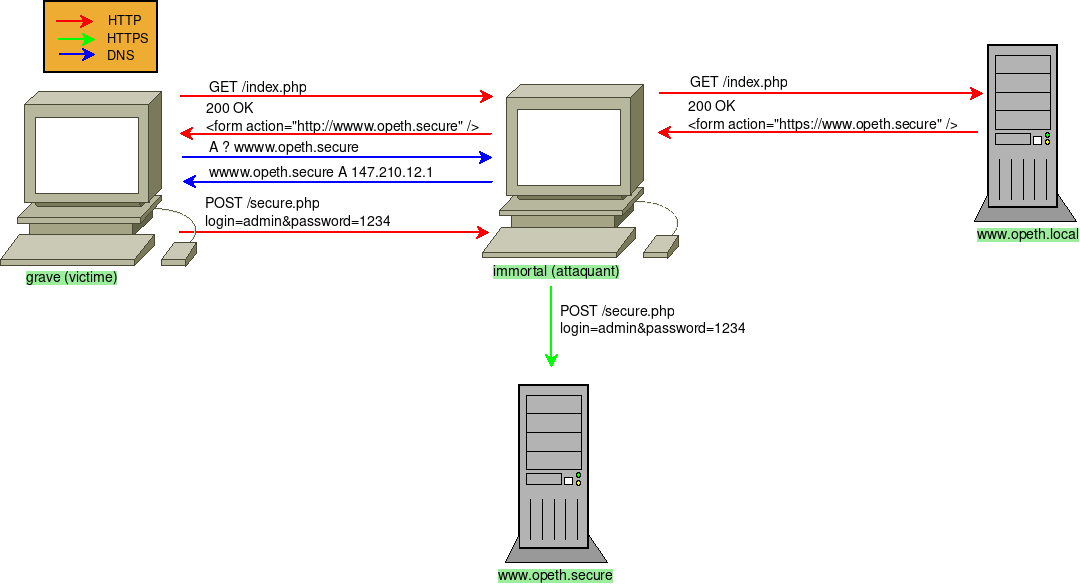
\includegraphics[width=\textwidth]{../medias/sslstrip2/attack.png}}
\end{figure}

Comme vu précédemment, une contre-mesure a été mise en place afin de déclarer aux clients d'un serveur qu'ils doivent utiliser une connexion sécurisée en HTTPS pour leur futures connexions avec celui-ci. Vous pouvez vous reporter à la section \hyperref[sec:hsts]{Contremesures} pour plus de précision.

Notre but est donc de contourner le HSTS en réutilisant l'attaque SSLStrip. Malheureusement, on ne peut pas la réutiliser directement car le navigateur a gardé en mémoire que toutes connexions sur cette page doivent se faire en HTTPS.

\section{Description de l'attaque}
Cette extension de SSLStrip a été pensée par LeonardoNve. Elle permet donc de passer au travers l'une des nouvelles contre-mesures mise en place sur les navigateurs. En effet, si l'attaquant se place en homme du milieu, il va pouvoir intercepter le trafic entre le client et le serveur afin de le faire réagir comme suit.

Lorsque le client va se connecter au serveur sur une page HTTP, l'attaquant va modifier cette page en remplaçant tous les liens HTTPS en HTTP mais aussi en changeant le nom de domaine. Changer le nom de domaine changera le comportement du navigateur. En effet, comme le navigateur ne connaît pas ce nom de domaine, il n'enverra pas d'exception liée à HSTS.

Voici un exemple :

Si le lien est \path{https://www.domain.secure}, on peut le remplacer par \path{http://wwww.domain.secure}.

Il faut noter que l'on enlève le \verb+s+ de \verb+https+ et que l'on remplace \verb+www+ par \verb+wwww+ ce qui change bien le nom de domaine.

Ainsi, l'attaquant fait croire au navigateur que cette requête est légitime et que \path{wwww.domain.secure} correspond au serveur distant. La connexion sera donc en HTTP et donc en clair.

\section{Notre attaque}

Tout d'abord, afin de pouvoir mettre en place l'attaque, il nous faut configurer l'environnement. Rappelons que l'attaquant est déjà positionné en homme du milieu, et que nous avons choisi de mettre sa machine dans le même réseau que la machine victime. Comme pour l'attaque précédente, nous utilisons l'outil \verb+qemunet+ développé par l'Inria qui nous permet de créer un environnement minimaliste et léger. Il nous faut donc vous expliquer sa mise en place.

\subsection{Mise en place de l'environnement}

Dans un premier temps, nous devons créer une topologie, c'est à dire un fichier décrivant l'architecture de l'environnement, qui correspond à notre besoin. En effet, nous avons besoin de trois machines :

\begin{itemize}
\item une machine cliente et victime
\item une machine attaquante
\item une machine serveur
\end{itemize}

Voici le fichier de topologie qui décrit l'environnement mis en place pour l'attaque.

\inputminted[bgcolor=lbcolor, breaklines]{shell}{../sslstrip2/topology}

Afin d'utiliser \verb+qemunet+ facilement, nous avons décidé de structurer l'environnement de l'attaque grâce à la gestion de dossiers supportée par l'outil. C'est pourquoi, tout l'environnement de l'attaque se trouve dans le dossier \verb+sslstrip2+ de notre projet. Ce dossier étant lui-même réparti en sous-dossiers. Chaque sous-dossier représente chaque machine :

\begin{itemize}
\item grave : dossier de la machine cliente et victime
\item immortal : dossier de la machine attaquante
\item opeth : dossier de la machine serveur
\end{itemize}

De plus, afin d'avoir une configuration qui est chargée à chaque lancement du système, nous utilisons des scripts bash \verb+start.sh+ qui sont chargés par \verb+qemunet+ au démarrage de chaque machine.

Maintenant, il nous faut décrire ces fichiers de lancement.

\subsubsection{Configuration de la machine cliente - grave - 147.210.13.2}
Cette machine se nomme grave et utilise un environnement graphique de la distribution Linux Alpine. Un navigateur Firefox est présent pour la démonstration ultérieure.

Pour que la machine puisse accéder au réseau, nous devons lui spécifier une adresse IP, son masque de sous-réseau ainsi que sa route par défaut.

Mais, dans le cadre de l'attaque, il faut aussi les informations pour la résolution du nom de domaine en rapport avec l'adresse IP du serveur. Nous en reparlerons plus en détail ultérieurement.

De plus, comme nous allons utiliser du HTTPS, il nous a fallût créer des certificats reconnus par le navigateur client. Pour cela, il nous est nécessaire d'ajouter le certificat dans les fichiers configuration de Firefox afin qu'il le considère comme de confiance.

\inputminted[bgcolor=lbcolor, breaklines]{shell}{../sslstrip2/grave/start.sh}

\subsubsection{Configuration de la machine serveur - opeth - 147.210.12.1}

Opeth représente notre serveur qui utilise le système d'exploitation debian.

Cette machine héberge un serveur HTTP(S) grâce à NGINX sur le port 80 et 443. Pour cela, nous avons créé un certificat utilisé pour les connexions HTTPS. Il a été généré avec \verb+openssl+ grâce aux scripts présents dans le dossier \path{CA}, et signé par notre autorité de certification. C'est pourquoi, dans un premier temps, nous avons implémenté un script qui créer cette autorité de certification :

\inputminted[bgcolor=lbcolor, breaklines]{shell}{../CA/create-ca.sh}

Ensuite, nous pouvons enfin créer le certificat pour les connexions HTTPS :

\inputminted[bgcolor=lbcolor, breaklines]{shell}{../CA/new-cert.sh}

De plus, comme sur les autres machines, nous avons un script de démarrage qui sur cette machine nous permet de lancer les services nécessaire pour l'attaque. Voici le script :

\inputminted[bgcolor=lbcolor, breaklines]{shell}{../sslstrip2/opeth/start.sh}

Comme on peut le voir, nous avons besoin d'utiliser du PHP pour un petit script de connexion à une page.

\inputminted[bgcolor=lbcolor, breaklines]{shell}{../sslstrip2/opeth/php7.0-fpm.conf}

Ensuite, on peut s'intéresser à la configuration de notre serveur NGINX. On doit lui spécifier :

\begin{itemize}
\item que l'on va utiliser du HTTP et du HTTPS
\item les certificats à utiliser
\item le chemin vers les pages non-sécurisées et vers celles sécurisées
\item que l'on utilise du PHP sur certaines pages
\item que l'on utilise le header HSTS
\end{itemize}

On a donc le fichier suivant \path{sslstrip2/opeth/nginx.conf} :

\inputminted[bgcolor=lbcolor, breaklines]{shell}{../sslstrip2/opeth/nginx.conf}

Enfin, on a besoin de définir un serveur DNS avec l'outil DNSMASQ. Le fichier \path{sslstrip2/opeth/dnsmasq.conf} spécifie notre nom de domaine et les actions relatives à la résolution du nom de domaine.

\inputminted[bgcolor=lbcolor, breaklines]{shell}{../sslstrip2/opeth/dnsmasq.conf}

On obtient donc le script de lancement suivant qui charge toutes les configurations et associe l'adresse IP de opeth au nom de domaine suivants :

\begin{itemize}
\item \path{www.opeth.local} lorsque l'on accède en HTTP à la page
\item \path{www.opeth.secure} lorsque l'on accède en HTTPS
\end{itemize}

\inputminted[bgcolor=lbcolor, breaklines]{shell}{../sslstrip2/opeth/start.sh}

\subsubsection{Configuration de la machine attaquante - immortal}

Cette machine présente deux adresses IP, une dans le réseau de la machine victime et l'autre dans celle du serveur afin d'être en position d'homme du milieu. Dans le cadre de l'attaque, nous l'avons configurée afin qu'elle relaie les paquets entre grave et opeth. Nous avons aussi configuré un serveur DNS sur cette machine afin de pouvoir rediriger les requêtes sur le bon serveur en fonction de si l'attaque est en cours ou non. Nous avons donc le script de démarrage de la machine suivant :

\inputminted[bgcolor=lbcolor, breaklines]{shell}{../sslstrip2/immortal/start.sh}

Ainsi que la même configuration du serveur DNS que pour opeth.

Comme précisé dans la description de l'attaque, nous avons besoin d'un nom de domaine supplémentaire afin de rediriger les requêtes DNS dessus. Ce nom de domaine est \path{wwww.opeth.secure}. On n'a donc besoin d'un règle dans la table PREROUTING de iptables afin de rediriger les paquets sur son propre serveur lorsque l'attaque à lieu.

Comme cette machine est positionnée en homme du milieu, c'est celle-ci qui contient la preuve de concept de l'attaque. Elle se trouve dans le fichier \path{/mnt/host/attack.sh}.

\inputminted[bgcolor=lbcolor, breaklines]{shell}{../sslstrip2/immortal/attack.sh}

Nous commençons par rediriger les requêtes HTTP (port 80) sur le port de notre proxy (port 4242), puis les requêtes DNS sont redirigées vers le serveur DNS de l'attaquant.

\subsection{Démonstration}

Après ces présentations de mise en place, nous pouvons vous montrer le fonctionnement de l'attaque via une démonstration. Pour lancer l'environnement de test, il faut utiliser la commande suivante (on aura récupéré préalablement le dépôt \textbf{qemunet}) :

\begin{minted}{bash}
  ./qemunet/qemunet.sh -x -S sslstrip2
\end{minted}

Maintenant, nous avons les trois machines de lancées. Les login et mot de passe sont :

\begin{itemize}
\item grave : toto - toto
\item immortal : root - rien
\item opeth : root - rien
\end{itemize}

\subsubsection{Étape 1 : Avant l'attaque}

Avant de vous montrer ce qu'il se passe lors de l'attaque, nous devons vous montrer l'état initial.

Lorsque l'attaque n'est pas lancée, nous pouvons voir sur la machine grave que la communication se passe sans problèmes et que la requête POST passe bien en HTTPS; immortal est donc incapable de voir les identifiants envoyés :

\begin{figure}[H]
  \caption{Attaque SSLstrip2 (avant l'attaque)}
  \fbox{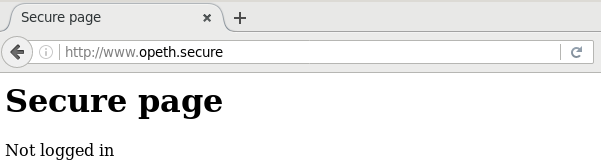
\includegraphics[width=\textwidth]{../medias/sslstrip2/screen1.png}}
\end{figure}

L'encadré rouge ci-dessous montre bien que le POST est effectué en HTTPS, sur le domaine \path{www.opeth.secure}. Lorsque nous affichons le code source de la page, nous obtenons :

\begin{figure}[H]
  \caption{Code source de la page (avant l'attaque)}
  \fbox{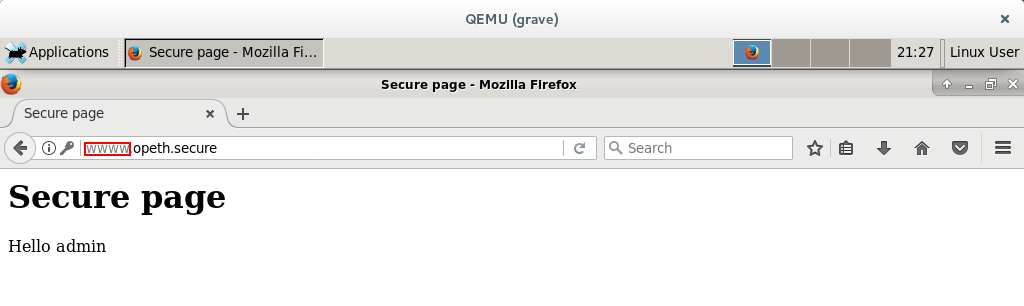
\includegraphics[width=\textwidth]{../medias/sslstrip2/screen2.png}}
\end{figure}

Nous arrivons alors sur le domaine \path{www.opeth.secure} en HTTPS : immortal n'a pas pût voir nos échanges sur cette page sécurisée comme le montre la figure ci-dessous.

\begin{figure}[H]
  \caption{La connexion se fait bien en https}
  \fbox{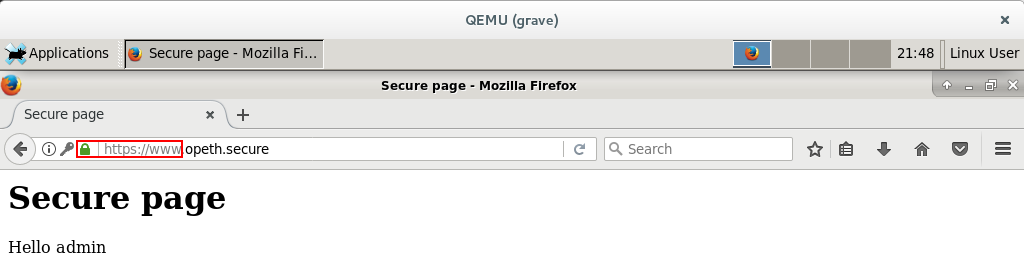
\includegraphics[width=\textwidth]{../medias/sslstrip2/screen3.png}}
\end{figure}

\subsubsection{Étape 2 : lancement de l'attaque}

Comme expliqué précédemment, pour lancer l'attaque, il faut exécuter le fichier \path{/mnt/host/attack.sh} depuis immortal dont on a déjà expliqué son comportement.

Nous pouvons maintenant lancer l'attaque depuis la machine immortal :


\begin{figure}[H]
  \caption{Lancement de l'attaque}
  \fbox{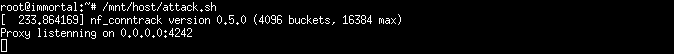
\includegraphics[width=\textwidth]{../medias/sslstrip2/screen4.png}}
\end{figure}

\paragraph{Explication du code \\}

Le code du proxy est dans le dossier de la machine immortal, le fichier \path{sslstrip2.py}.

\subparagraph{Réception des requêtes \\}

Lors de la réception de requêtes, il s'agit de savoir si l'on doit :

\begin{itemize}
\item fermer la connexion (le client ou le serveur a fermé la connexion)
\item établir une connexion en HTTPS, dans le cas où le client va sur le domaine \path{wwww.opeth.secure}
  \item établir une connexion HTTP, dans le cas où le client demande la page du domaine \path{www.opeth.local}
\end{itemize}

La fonction traitant les différentes requêtes est celle-ci :

\begin{minted}{python}
def __recv(self, csock):
        fw_sock = self.__csockets[csock]
        data = csock.recv(BUFFER_SIZE)
        if len(data) == 0:
            self.__close_conn(csock)
            self.__close_conn(fw_sock)
        else:
            print(data)

            if fw_sock is None:
                m = re.search(b'Host: (\S+)', data)
                if m is not None and m.group(1) == FAKE_HOST:
                    re.sub(b'Host: (\S+)',
                           b'Host: ' + bytes(FORWARD_HOST_HSTS), data)
                    self.__new_https_conn(csock)
                else:
                    self.__new_http_conn(csock)
                fw_sock = self.__csockets[csock]
            data = self.__replace_https_to_http(data)
            data = self.__replace_host(data)
            data = self.__replace_content_length(data)
            fw_sock.send(data)
\end{minted}

À la fin, on transforme tous les liens HTTPS trouvés en HTTP en remplaçant le nom de domaine \path{www.opeth.secure} par le faux nom de domaine \path{wwww.opeth.secure}, on met l'entête Host vers le bon domaine et on recalcule la taille de la requête (entête Content-Lenght)

\subparagraph{Transformation des liens \\}

Dans cette fonction, nous utilisons une expression régulière afin de remplacer tous les liens \path{https://www.opeth.secure} en \path{http://wwww.opeth.secure}.

\begin{minted}{python}
def __replace_https_to_http(self, data):
    return re.sub(b'https://' + bytes(FORWARD_HOST_HSTS),
                  b'http://' + bytes(FAKE_HOST), data)
\end{minted}

\subparagraph{Modification de l'entête Host}

Lorsque la victime est redirigée vers un lien \path{http://wwww.opeth.secure}, l'entête Host de ses requêtes sera erronée. Cette fonction modifie cette entête pour que le serveur puisse recevoir un Host correct.

\begin{minted}{python}
def __replace_host(self, data):
    return re.sub(b'Host: ' + bytes(FAKE_HOST),
                  b'Host: ' + bytes(FORWARD_HOST_HSTS), data)
\end{minted}


\subparagraph{Recalcul de l'entête Content-Length}

La taille de la requête étant modifiée par le proxy, celui-ci doit recalculer l'entête Content-Length en se basant sur la chaîne "{\textbackslash}r{\textbackslash}n{\textbackslash}r{\textbackslash}n" signalant la fin des entêtes dans le protocole HTTP.

\begin{minted}{python}
def __replace_content_length(self, data):
    try:
        idx = data.index(b"\r\n\r\n")
        length = len(data) - idx - 4
        return re.sub(b'Content-Length: (\d+)',
                      b'Content-Length: %d' % length, data, 1)
    except:
        return data
\end{minted}

\subsubsection{Étape 3 : Pendant l'attaque}

Lorsque l'attaque est lancée, on peut voir que le lien sensible \path{https://www.opeth.secure} est remplacé par \path{http://wwww.opeth.secure}.
La machine immortal est donc capable d'intercepter les échanges réalisés sur le domaine \path{www.opeth.secure}.

Dans cette image, on voit dans l'encadré rouge, que le lien \path{https://} a bien été remplacé par un lien non sécurisé \path{http://} :

\begin{figure}[H]
  \caption{Le 's' de "https" a disparu}
  \fbox{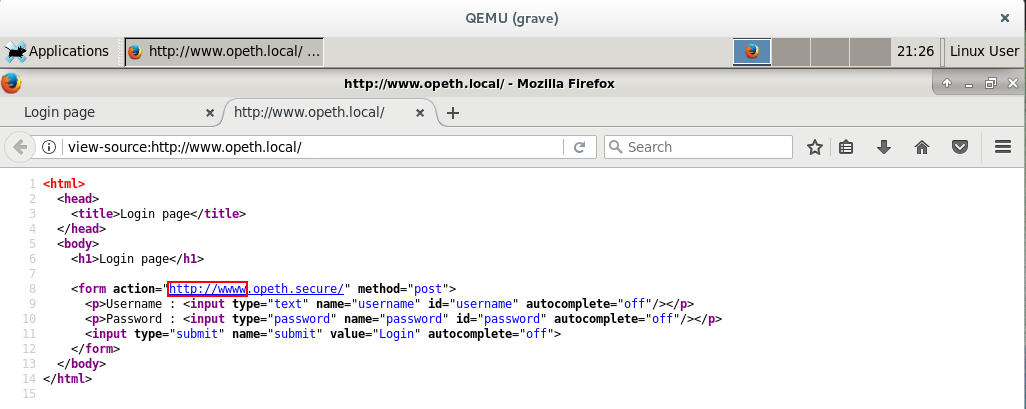
\includegraphics[width=\textwidth]{../medias/sslstrip2/screen5.png}}
\end{figure}

Nous constatons que nous arrivons sur la page secure.php en HTTP : notre navigation n'est pas sécurisée !

\begin{figure}[H]
  \caption{Le client visite une page sécurisée en http}
  \fbox{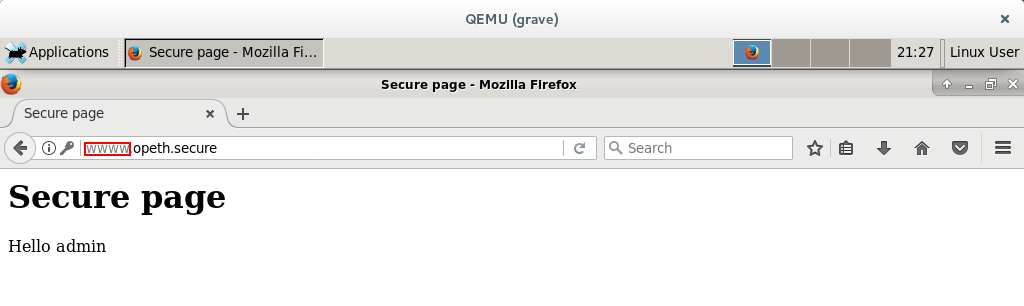
\includegraphics[width=\textwidth]{../medias/sslstrip2/screen6.png}}
\end{figure}

La machine immortal a été capable de capturer non seulement les identifiants du formulaire, mais également le cookie de session :

\begin{figure}[H]
  \caption{L'attaquant récupère toutes les informations sensibles}
  \fbox{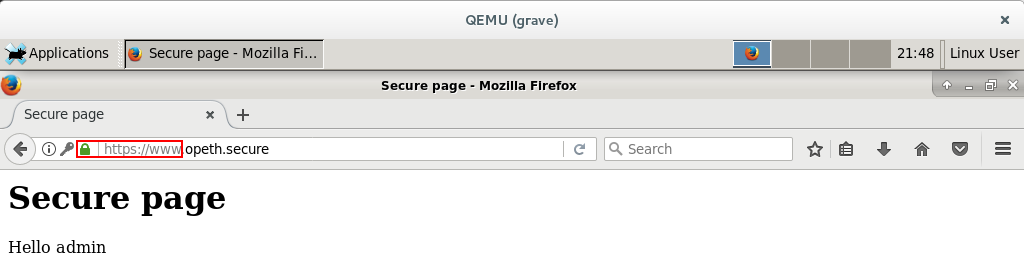
\includegraphics[width=\textwidth]{../medias/sslstrip2/screen7.png}}
\end{figure}
